\section{Evaluation}\label{eval}

%V.	Evaluation
%	a.	Models
%		i.	Model Accuracy
%			1.	Matlab
%		ii.	Performance/Overhead
%			1.	Tess
%				a.	Time to build the model
%				b.	Phase Change Reaction
%		i.	Video Application adding threads
%		ii.	Time to react to phase changes
%		iii.	Show model accuracy through transition?
%	b.	Decisions
%		i.	Decision Accuracy
%			1.	Matlab
%		ii.	Performance/Overhead
%			1.	Tess
%	c.	Dynamic System
%		i.	Single Application � right sizing
%			1.	Without phase changes
%			2.	With phase changes
%			3.	Baseline � all allocations
%			4.	Measure Energy
%		ii.	Video, Animation, and Throughput Applications w/o phase changes
%			1.	Show throughput and missed deadlines for all the possible mixes
%			2.	Is it possible to show optimal?
%			3.	What is the baseline?
%		iii.	Video, Animation, and Throughput Applications w/ phase changes
%			1.	Show throughput and missed deadlines for all the possible mixes
%			2.	Basically just to show the system works

In this section, we show the high-level results on how well \pacora performs resource allocation to illustrate the viability of \pacora before diving into all the system details in the following sections.   Evaluations of the performance of individual components of \pacora is included with the detailed technical descriptions of the components.

We use two different implementations of the \pacora framework for evaluation. Our static framework collects data online using an x86 processor running Linux.  That data is then used to build models and make and evaluate static resource allocation decisions.  Our static framework was used to experiment with the accuracy of different types of models and test the quality of the resource allocation decisions.  Our dynamic framework is implemented in a research operating system, \tess, and is used to test our implementations of the algorithms, measure the overhead and reaction times, and illustrate \pacora's ability to work in a real system.

\subsection*{Static Resource Allocation Framework}
Our static framework was designed to test the effectiveness of \pacora's model-based convex optimization for allocating resources.  Data is collected online by running application benchmarks on a recent x86 processor running Linux-2.6.36.  The measured data is processed using Python and then fed to MATLAB~\cite{matlab} to build the RTFs.  MATLAB uses the RTFs to make resource allocation decisions.  We compare performance of the chosen resource allocations with the actual measured performance of all possible resource allocations to test quality of the resource allocation decisions. We use CVX~\cite{cvx} in MATLAB to perform the convex optimization for building RTFs and making resource allocation decisions.  We used this approach because it enabled us to test many applications, 44 in total, and many resource allocations rapidly.

\subsubsection*{Platform}

To collect data, we use a prototype version of Intel's Sandy Bridge x86 processor that is similar to the
commercially available client chip, but with additional hardware
support for way-based LLC partitioning.
The Sandy Bridge client chip has 4 quad-issue out-of-order
superscalar cores, each of which supports 2 hyperthreads using
simultaneous multithreading~\cite{IntelRefManual:2011}.  Each core has
private \wunits{32}{KB} instruction and data caches, as well as a
\wunits{256}{KB} private non-inclusive L2 cache.  The LLC is a 12-way
set-associative \wunits{6}{MB} inclusive L3 cache, shared among all
cores using a ring-based interconnect.  All three cache levels are
write-back.   The cache partitioning mechanism is way-based and works by modifying the
cache-replacement algorithm.  To allocate cache ways, we assign a subset of
the 12 ways to a set of hyperthreads, thereby allowing only those hyperthreads to replace data in those ways.

%Way allocations can be completely private,
%completely shared, or overlapping.  Although all cores can hit on data stored in
%any way, a core can only replace data in its assigned
%ways.   Data is not flushed when the way allocation changes.

We use a customized BIOS that enables the cache partitioning
mechanism, and run unmodified Linux-2.6.36 for all of our experiments.
To allocate cores, we use the Linux {\tt taskset} command to pin applications to
sets of hyperthreads.  For our experiments we consider each hyperthread to be an independent core. To minimize the interference between hyperthreads, we first assign both hyperthreads available in one core before moving on to the next core. For example, allocations with four cores correspond to running on both hyperthreads of two cores.

\subsubsection*{Performance and Energy Measurement}

To measure application performance, we use the \texttt{libpfm}
library~\cite{Eranian:OLS06,Perfmon2}, built on top of the
\texttt{perf\_events} infrastructure introduced in Linux 2.6.31, to
access available performance counters~\cite{Intel:Manual2012}.

To measure on-chip energy, we use the energy counters available on
Sandy Bridge to measure the consumption of  the entire socket and also
the total combined energy of cores, their private caches, and the
LLC. We access these counters using the Running Average Power Limit
(RAPL) interfaces~\cite{Intel:Manual2012}.  The counters measure power
at a $1/2^{16}$ second granularity.

%In addition, we use a FitPC external multimeter to measure at the wall socket the power
%consumed by the entire system, at a
%\wunits{1}{second} granularity.
%We correlate the wall power data with the data collected from the hardware energy counters
%using time stamps.  We observed less than one second of delay in these
%measurements consistently across all experiments.  Together, these
%mechanisms allow us to collect accurate energy readings over the
%entire course of an application's execution.

\subsubsection*{Description of Workloads}

Our workload contains a range of applications from three different
popular benchmark suites: SPEC CPU 2006~\cite{SPEC2006},
DaCapo~\cite{dacapo}, and PARSEC~\cite{parsec}. We selected this set of applications to represent a wide variety of possible resource behaviors in order to properly stress \pacora's RTFs. We include some additional applications to broaden the
scope of the study, and some microbenchmarks to exercise certain
system features.

The \textbf{SPEC CPU2006} benchmark suite~\cite{SPEC2006} is a
CPU-intensive, single-threaded benchmark suite, designed to stress a
system's processor, memory subsystem and compiler.  Using the
similarity analysis performed by Phansalkar et
al.~\cite{Phansalkar:ISCA2007}, we subset the suite, selecting 4
integer benchmarks ({\tt astar}, {\tt libquantum}, {\tt mcf}, {\tt omnetpp}) and 4
floating-point benchmarks (cactusADM, calculix, lbm, povray).  Based
on the characterization study by Jaleel~\cite{Jaleel:TR2007}, we also
pick 4 extra floating-point benchmarks that stress the LLC: {\tt GemsFDTD},
{\tt leslie3d}, {\tt soplex} and {\tt sphinx3}.  When multiple input sets and sizes are
available, we pick the single \textit{ref} input indicated by
Phansalkar et al.~\cite{Phansalkar:ISCA2007}.

We include the \textbf{DaCapo} Java benchmark suite as a
representative of a managed-language workloads. We use the latest 2009 release, which consists of a set of open-source, real-world
applications with non-trivial memory loads, and includes both client and
server-side applications.

The \textbf{PARSEC} benchmark suite is intended to be representative
of parallel real-world applications~\cite{parsec}. PARSEC
programs use various parallelization approaches, including data- and
task-parallelization. We use native input sets and the {\tt pthreads} version for all benchmarks, with the exception of
\texttt{freqmine}, which is only available in OpenMP.

We add four \textbf{additional parallel applications} to help ensure
we cover the space of interest: {\tt Browser\_animation} is a
multithreaded kernel representing a browser layout animation; {\tt
  G500\_csr} code is a breadth-first search algorithm; {\tt Paradecoder} is a parallel
speech-recognition application that takes audio waveforms of human
speech and infers the most likely word sequence intended by the
speaker; {\tt Stencilprobe} simulates heat transfer in a fluid
using a parallel stencil kernel over a regular
grid~\cite{Kamil:Stencilprobe}.

We also add two \textbf{microbenchmarks} that stress the memory
system: {\tt stream\_uncached} is a memory and on-chip bandwidth hog
that continuously brings data from memory without caching it, while
{\tt ccbench} explores arrays of different sizes to determine the
structure of the cache hierarchy.

Using a performance characterization of the applications, we select a subset of the benchmarks that are representative of different possible responses to resource allocations in order to reduce our study to a feasible size.  Similar to \cite{Phansalkar:ISCA2007}, we use machine learning to select representative benchmarks.  We use a
hierarchical clustering algorithm~\cite{Phansalkar:ISCA2007} provided by the Python library \texttt{scipy-cluster} with the \textit{single-linkage} method.  The feature vector contains parameters to represent core scaling, cache scaling, prefetcher sensitivity and bandwidth sensitivity.  The clustering algorithm uses Euclidean distance between vectors to determine clusters.

The clustering results in 6 clusters representing the following (applications at the cluster center are listed in parenthesis):
 \begin{itemize}\itemsep0pt \parskip0pt \parsep5pt
\item no scalability, high cache utility, ({\tt 429.mcf})
\item no scalability, low cache utility, ({\tt 459.gems\-FDTD})
\item high scalability, low cache utility, ({\tt ferret})
\item limited scalability, high cache utility, ({\tt fop})
\item limited scalability, low cache utility, ({\tt dedup})
\item limited scalability, low bandwidth sensitivity, ({\tt batik})
\end{itemize}

%First, we create a feature vector for each application using the values in the previous subsection:
%1) execution time as we increase the number of threads; 2) execution time as we increase the LLC size; 3) prefetcher sensitivity; and 4) bandwidth sensitivity. All metrics are normalized to the interval $[0,1]$. In total we use vectors with 19 features ($7+10+1+1$).

%The clustering algorithm finds the smallest Euclidean distance of a pair of feature vectors and forms a cluster containing that pair. It continues selecting the next smallest distance between a pair and forms another cluster. Linkage criteria can be used to adjust cluster formation. The single-linkage we selected uses the minimum distance between a pair of objects in different clusters to determine the distance between them.

\subsubsection*{RTF Experiments}
\begin{figure*}[!t]
	\begin{center}	
		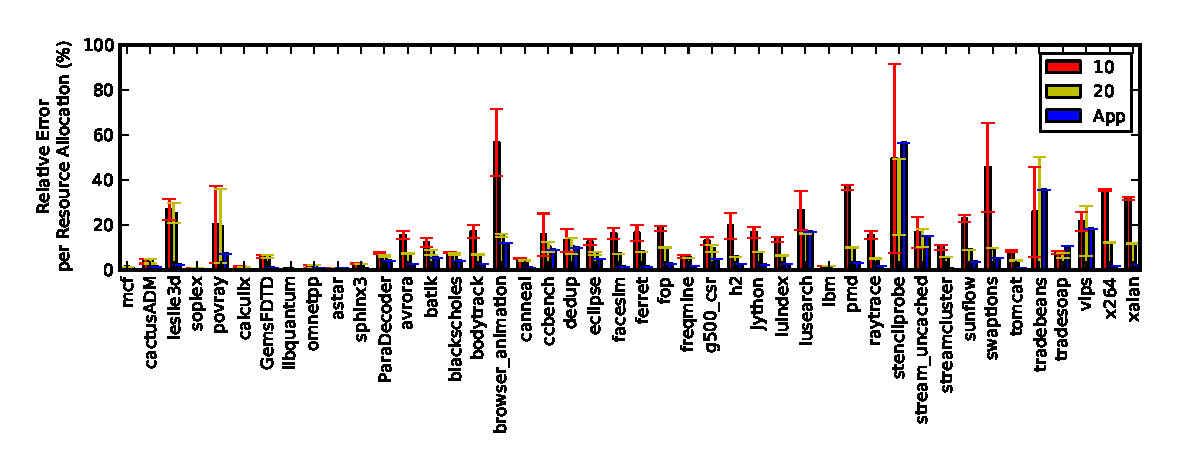
\includegraphics[width=1.0\textwidth]{model_accuracy.pdf}
		\caption{L1 norm of relative error from RTF predicted response time compared to actual measured response time.  Data represents the average error from 3 trials.}
		\label{model_accuracy}
	\end{center}
\end{figure*}
To test the effectiveness of our RTFs in capturing real application behavior, we measured each of our 44 total benchmarks running alone on the machine for all possible resource allocations of cache and cores.  Cores can be allocated from 1-8 and cache from 1-12 resulting in 96 possible allocations for each application.   We use a genetic algorithm design of experiments~\cite{bates-aes03} to select 10 and 20 of the collected allocations to build the RTFs.  We also experimented with building RTFs with more data points but found that they provided little improvement over 20.  We then use the model to predict the performance of every resource allocation and compare it with the actual measured performance of that resource allocation.  We ran 3 complete trials and took the average error of the 3 trials.

Figure~\ref{model_accuracy} shows the L1 norm of relative error of the predicted response times.
% \fix{explain results, whats up with tradebeans, how do we know these are any good}.

\subsubsection*{Resource Allocation Experiments}
\begin{figure}[!t]
	\begin{center}	
		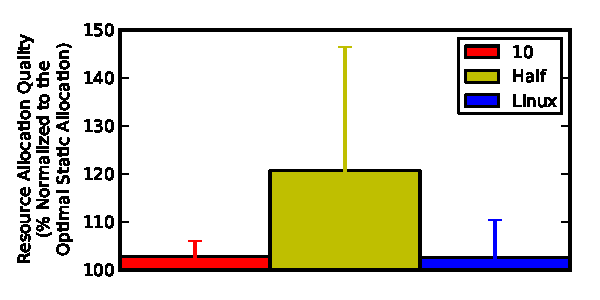
\includegraphics[bb=0 0 656 313,width=0.9\columnwidth]{decision_quality.pdf}
		\caption{Resource allocation decisions for each pair of the cluster representative applications compared with the optimal allocation, the Linux scheduler, and equally dividing the machine.}
		\label{cluster_decision_quality}
	\end{center}
\end{figure}

\begin{figure}[!t]
	\begin{center}	
		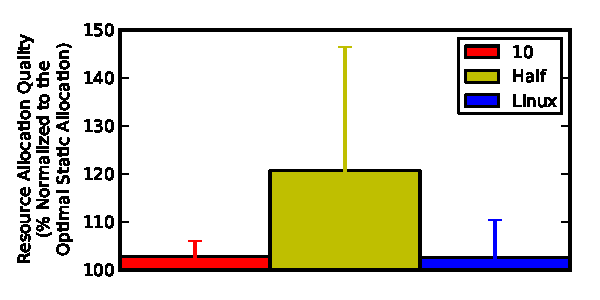
\includegraphics[bb=0 0 656 313,width=0.9\columnwidth]{decision_quality.pdf}
%		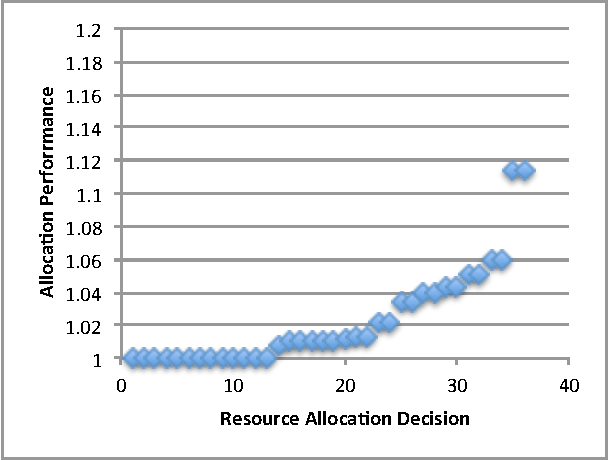
\includegraphics[width=.45\textwidth]{cluster_decision_points.pdf}
%		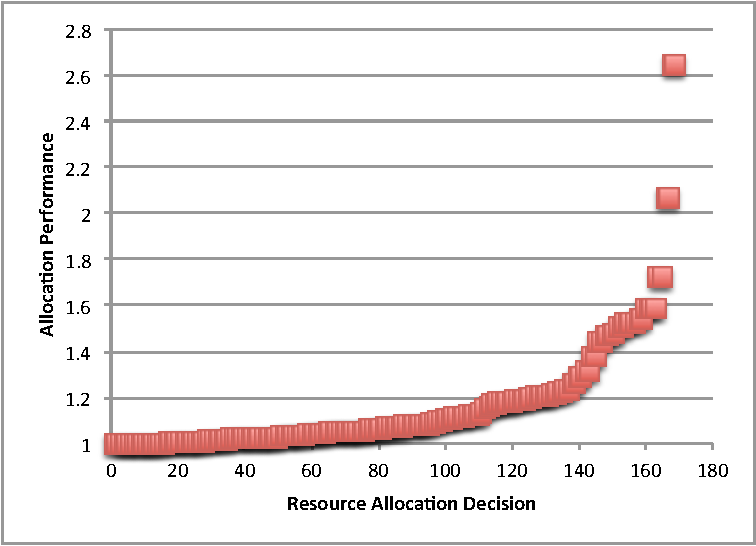
\includegraphics[width=.45\textwidth]{parsec_decision_points.pdf}
		\caption{Resource allocation decisions for each pair of PARSEC applications compared with the optimal allocation, the Linux scheduler, and equally dividing the machine.}
		\label{parsec_decision_quality}
	\end{center}
\end{figure}

Using the RTFs functions built for the applications, we have \pacora make static resource allocations for all possible pairs of the cluster representative applications.  We then run all possible resource allocations for each pair on our Sandy Bridge/Linux platform and collect the performance.  Using this data compare we compare the measured performance of \pacora's chosen allocation with the best performing, \emph{i.e.,} optimal, resource allocation.  We also compare the result to equally dividing the resources between the two applications and sharing all of the resources using the Linux scheduler.


Figure~\ref{cluster_decision_quality} shows how \pacora's decisions compared with the optimal allocation, the Linux scheduler, and equally dividing the machine for each pair of the cluster representative applications.  We also perform the same experiment for all pairs of PARSEC applications since they scale the better than the other benchmark suites thus enabling more viable resource allocations.  Figure~\ref{parsec_decision_quality} shows the results.

\subsection*{Dynamic Resource Allocation in a Manycore OS}
%\cite{tess09,tess_dac}
In order to evaluate \pacora's effectiveness dynamically making decisions in real-time in a real operating system, we implemented in an in-house research operating system, \tess. We chose to implement in \tess over Linux for two reasons:
 \begin{itemize}\itemsep0pt \parskip0pt \parsep5pt
\item \tess is designed around two-level scheduling meaning it more accurately reflects the system design \pacora assumes
\item \tess allows resource revocation, enabling \pacora to dynamically reallocate resources
\item \tess implements additional resource partitioning and QoS mechanisms allowing \pacora to explore allocating more resource types
\end{itemize}

\subsubsection*{Platform}
Our dynamic experiments are all run on an Intel Nehalem-EP system with two 2.66-GHz Xeon X5550 quad-core processors and hyperthreading enable (\emph{i.e.,} 16 hardware threads). It also contains a 1-Gbps Intel Pro/1000 Ethernet network adapter.
\tess allocates resources directly to applications and then applications employ a second-level scheduler to schedule threads onto the resources.  There are have two scheduling frameworks available in \tess, a cooperative framework called Lithe (LIquid THrEads)~\cite{lithe} and a preemptive one called PULSE (Preemptive User-Level SchEduling).  All of our experiments are run using 2 different schedulers in the PULSE framework; applications with responsiveness requirements use the EDF, earliest-deadline first, scheduler and throughput oriented applications use the GRR, global round-robin, scheduler.

\tess in addition to allocating cores and cache ways as with our static framework, \tess can also allocate fractions of network bandwidth.  In our experiments, we show \pacora allocating cores and network bandwidth because the experimental platform, which has the advantage of more cores, does not have cache partitioning.  We have also experimented with additional resources such as memory pages and cpu utilization, but they are not shown in this paper.

\subsubsection*{Performance and Energy Measurement}
Applications report their own measured response times to \pacora through a message-passing interface built into \tess.  \pacora uses this information to build models, and we also use this information to show if the application is making its deadlines for the experiments.

\tess enables \pacora to directly measure the system energy.  However, energy counters are not available on our Nehalem-EP system and thus we extend the power model from the Sandy Bridge system to function as our Application 0 RTF.

\subsubsection*{Description of Workloads}
Our workload is designed to represent the scenario of a video conference, where each participant requires a separate, performance guaranteed video stream.
New participants may join the conference and others leave, increasing or decreasing the number of streams running at any given time.  Additionally, the speaker's video is larger and higher resolution than the other video streams and as the speaker changes the requirements for video streams change. While conferencing, compute-intensive tasks, such as virus scans or file indexing, could be executed in background.

Our streaming video application is a multi-threaded, cpu- and network-intensive workload intended to simulate video chat applications like Skype and Facetime.
Each video stream is encoded offline in the H.264 format using libx264, transported across the network through a TCP connection, and decoded and displayed by the \tess client. The client receives, decodes and displays each frame using libffmpeg and libx264. Each video stream has a corresponding EDF-scheduled thread with 33 ms deadlines using our second-level EDF scheduler.

We use psearchy~\cite{psearchy}, a parallel text indexer, from MOSBENCH\cite{mosbench} as our file indexing application. We also use a network bandwidth hog application designed to contend with the video player for bandwidth by constantly sending UDP messages to the Linux box.

\subsubsection*{Resource Allocation Experiments}
\begin{figure*}[!t]
	\begin{center}	
%		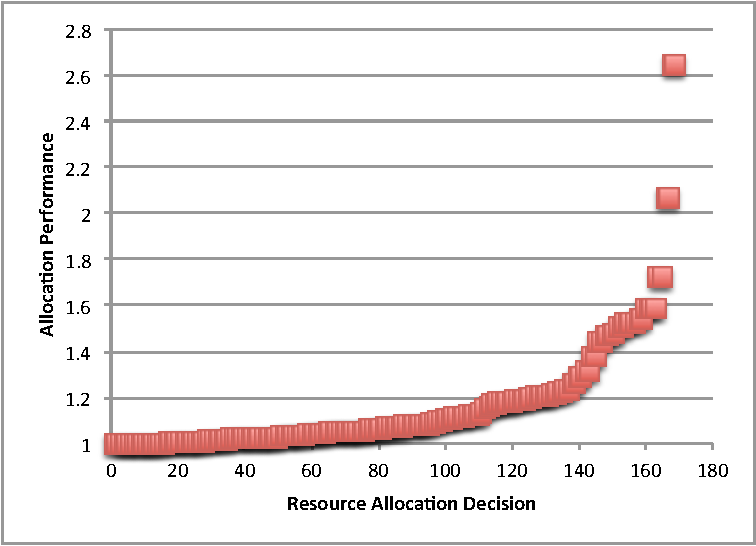
\includegraphics[width=.45\textwidth]{parsec_decision_points.pdf}
		\caption{Resource Allocations of video conferencing through time as participants enter and leave and the video in focus changes with the computer operating in wall power mode}
		\label{video_experiment_wp}
	\end{center}
\end{figure*}

\begin{figure*}[!t]
	\begin{center}	
%		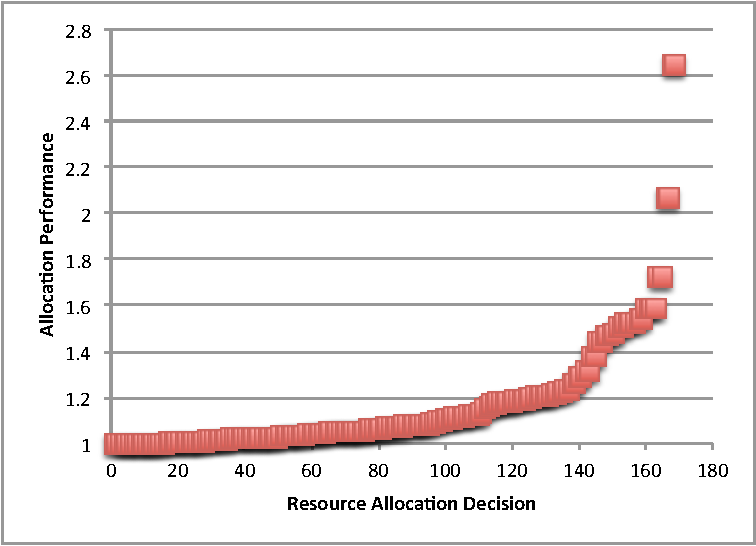
\includegraphics[width=.45\textwidth]{parsec_decision_points.pdf}
		\caption{Resource Allocations of video conferencing through time as participants enter and leave and the video in focus changes with the computer operating in battery power mode}
		\label{video_experiment_battery}
	\end{center}
\end{figure*}

Figure~\ref{video_experiment_wp} shows the resource allocations for our video conference scenario when the computer is using wall power. Figure~\ref{video_experiment_battery} shows same scenario except the computer is now using battery power and thus we have increased the importance of the wall.








